\documentclass[twocolumn, 8pt]{article}

\usepackage{lipsum}
\usepackage{JAMIA}

\title{My Cool Title Here}
\author[1, 2]{Author One, MD}
\author[2]{Author Two, PhD}
\author[1]{Author Three, PhD}
\affil[1]{Institution One, Country;}
\affil[2]{Institution Two, Country}
\date{}

\begin{document}

% make title and abstract
%==============================
\par\noindent\rule[-7pt]{15.5cm}{0.2em}
\begin{strip}
    \begin{minipage}{.88\textwidth}
        \maketitle
        \small
        \abstractSection
        {This is a cool work. Cool works must be accepted. So, accept this work.} % Objective
        {} % Materials and Methods
        {} % Results
        {} % Discussion
        {} % Conclusion
        {deep learning, machine learning} % Key words
        
        \par\noindent\rule[-7pt]{15.5cm}{0.2em}
        \hspace{2cm}
    \end{minipage}
\end{strip}
%==============================


% Introduction
%==============================
\section*{Introduction}

\begin{figure*}
    \centering
    \setlength{\abovecaptionskip}{0pt}
    % \includegraphics[width=0.9\textwidth, trim=1.7cm 7cm 8.5cm 2cm, clip]{img/figure1.pdf} % Could crop PDF
    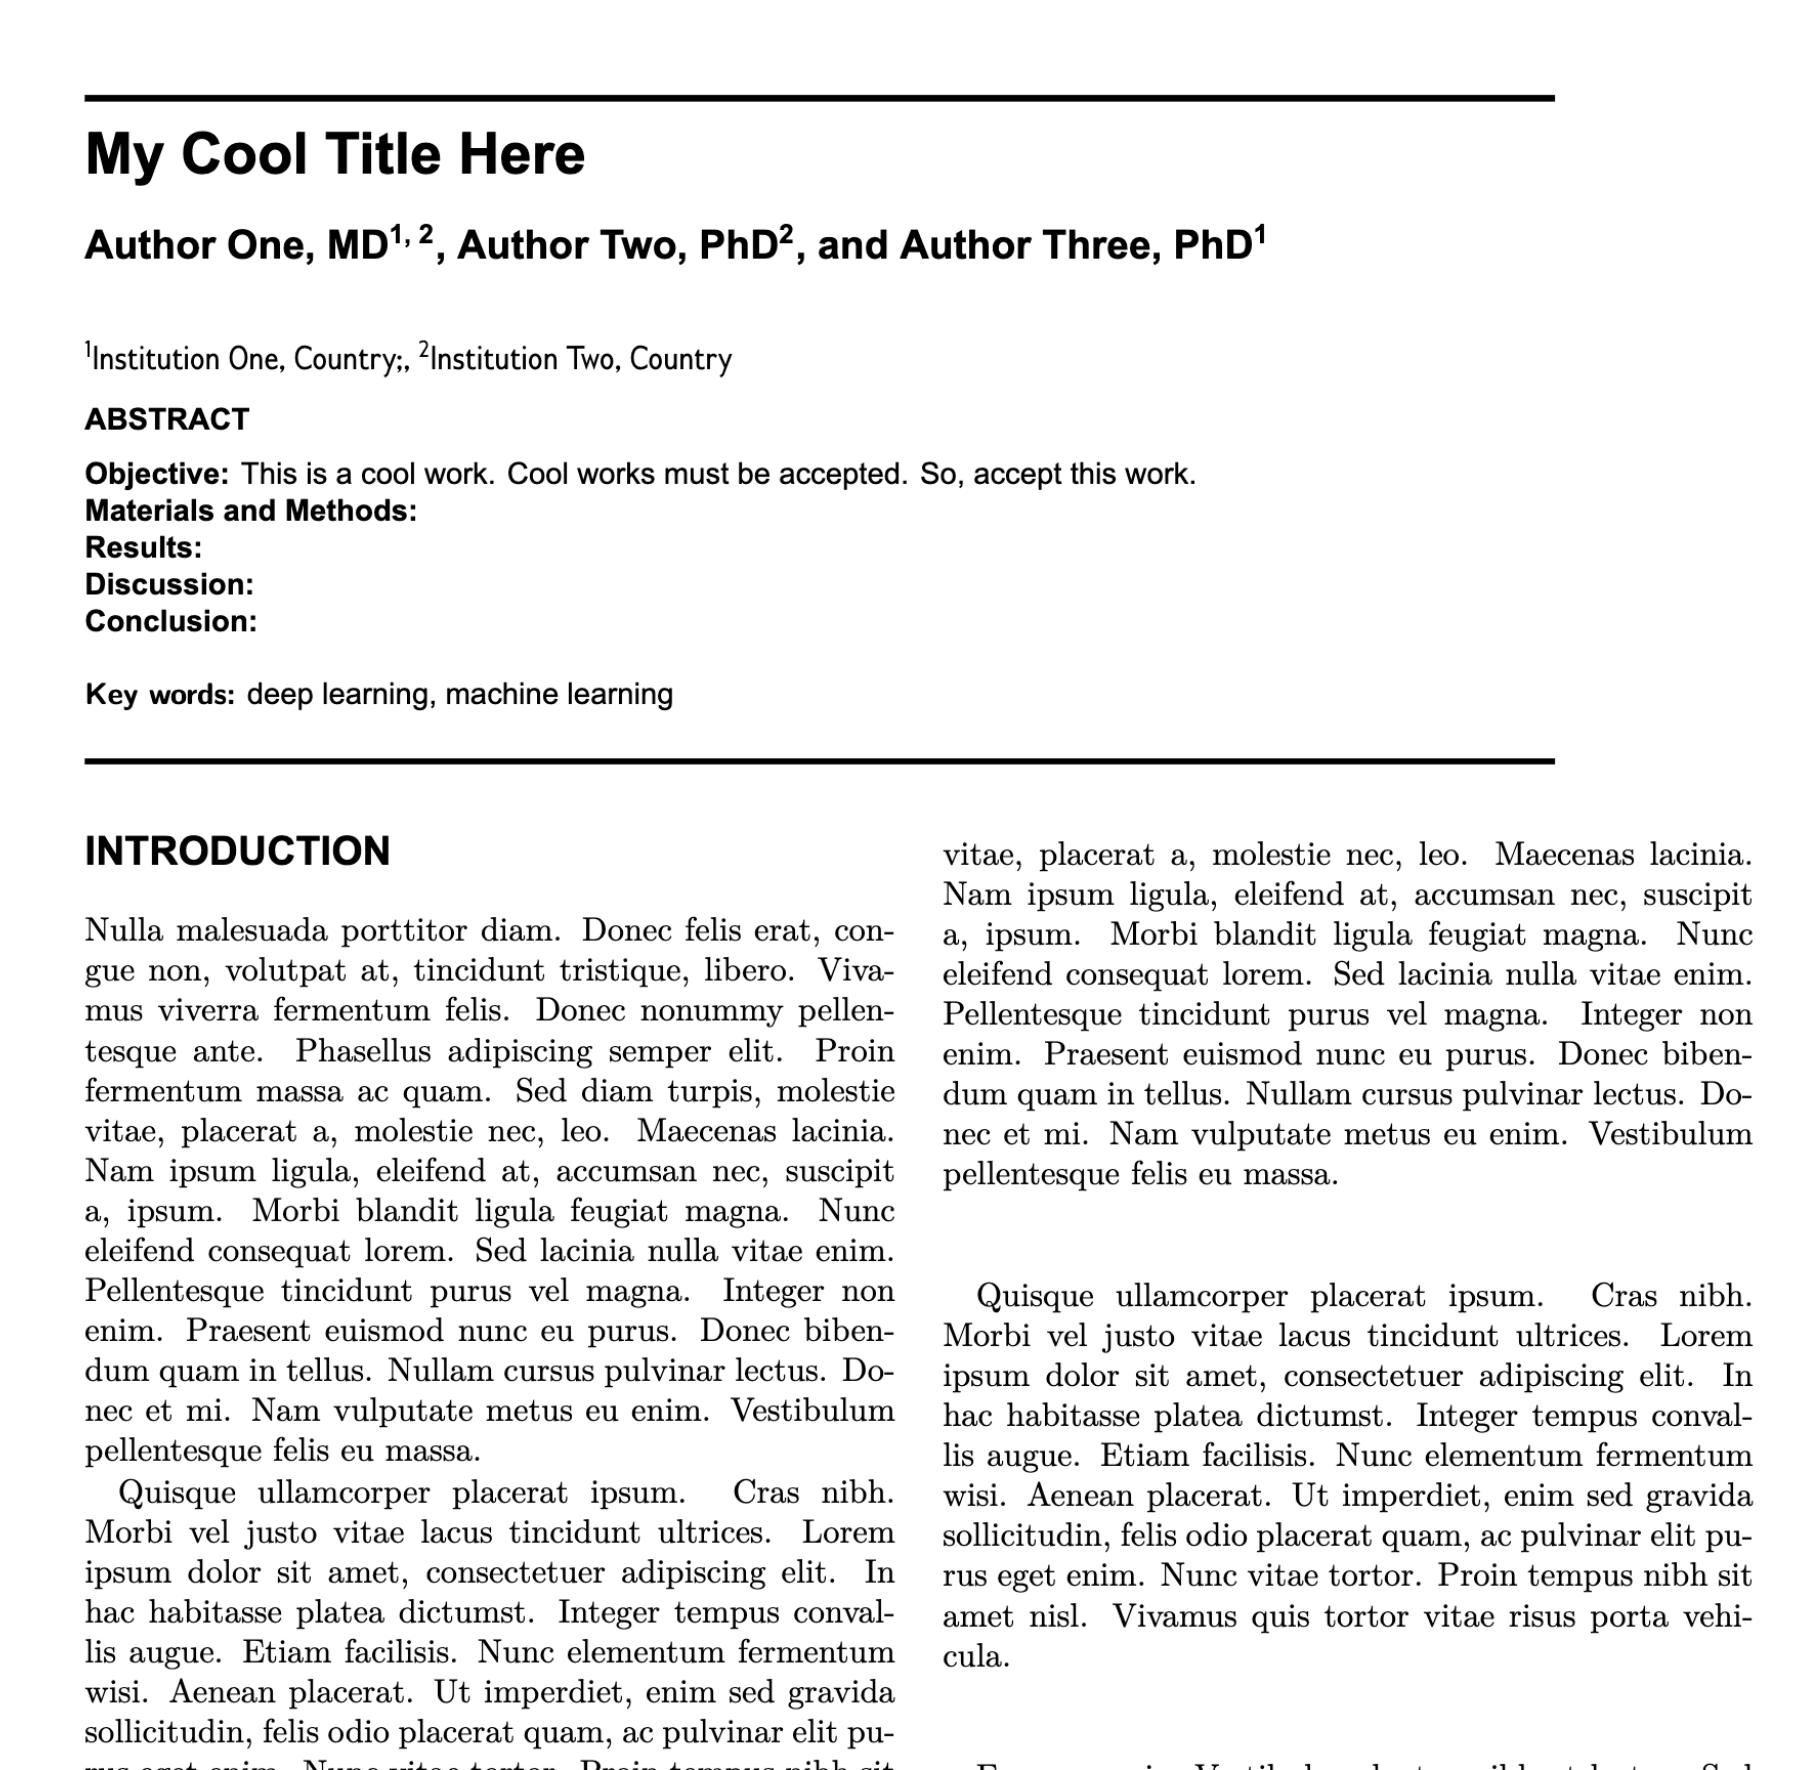
\includegraphics[width=0.4\textwidth]{img/example.png}
    \caption{This is a image.}
    \label{fig::local_pred_model}
\end{figure*}

\lipsum[3-8] \cite{he2016deep} \textcolor{red}{\textbf{CITE HERE!}}
%==============================

\begin{table*}[hbt!]
\setlength{\abovecaptionskip}{5pt}
\caption{This is Table 1.}
\label{tab::conv}
\centering
% \resizebox{\textwidth}{!}{
\resizebox{13cm}{!}{
    \begin{tabular}{lccccccc}
        \toprule
        & \multicolumn{7}{c}{\textbf{Table}} \\
        \cline{2-8}
        & \textbf{Table} & \textbf{Table} & \textbf{Table} & \textbf{Table} & \textbf{Table} & \textbf{Table} & \textbf{Table}\\
        \midrule
        \textbf{Table*} &&&&&& \\
        \quad \# Within 6 Table &  &  &  &  &  &  & \\
        \quad \# Within 12 Table &  &  &  &  &  &  & \\
        \cline{1-8}
        \# Average Table &  &  &  &  &  &  & \\
        \cline{1-8}
        \multicolumn{8}{l}{\small \quad*Table: table table}\\
    \end{tabular}
}
\end{table*}

\begin{table*}[hbt!]
\setlength{\abovecaptionskip}{5pt}
\caption{This is Table 2.}
\centering
\resizebox{13cm}{!}{
\begin{tabular}{cccccc}
    \toprule
    \textbf{Table} & \textbf{Table} & \textbf{Within 6 Table} & \textbf{Within 12 Table} & \textbf{Within 24 Table} & \textbf{No Table} \\ 
    \midrule
    \multirow{4}{*}{\textbf{Big Table}}   
        & Table &  &  &  &  \\
        & Table &  &  &  &  \\
        & Table &  &  &  &  \\
        & Table &  &  &  &  \\
    \cline{1-6}
\end{tabular}
}
\label{tab::reuslt}
\end{table*}

% Materials and Methods
%==============================
\section*{Materials and Methods}
\subsection*{Study overview}

\lipsum[3-9]
%==============================

% Results
%==============================
\section*{Results}

\lipsum[3] \textbf{Table \ref{tab::conv}}

\textbf{Table \ref{tab::reuslt}} \lipsum[4]
%==============================

% Discussion
%==============================
\section*{Discussion}

\lipsum[3-6]
%==============================

% Conclusion
%==============================
\section*{Conclusion}

\lipsum[3-4]
%==============================

% Funding
%==============================
\section*{Funding}
\lipsum[3-4]
%==============================

% Reference
%==============================
\bibliographystyle{vancouver}
{\footnotesize \bibliography{citiation}}
%==============================

\end{document} 